\begin{figure*}[t]
\centering
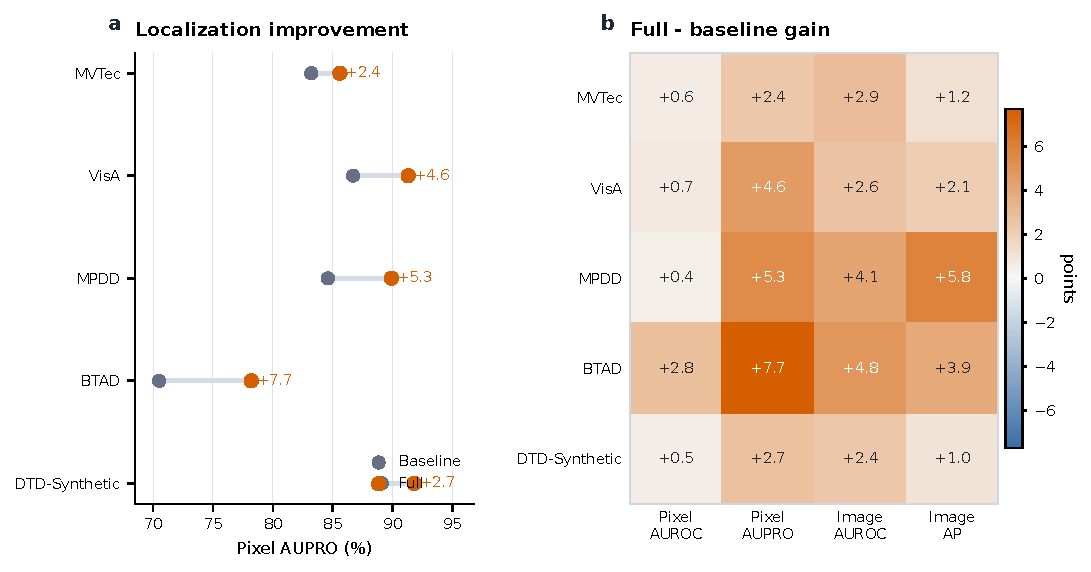
\includegraphics[width=\textwidth]{figures/figure1_main_results.pdf}
\caption{Main result summary across five anomaly detection datasets. (a) Pixel-level AUPRO comparison between the AnomalyCLIP baseline and the full method. Values on the right report absolute point gains. (b) Full-method gains over the baseline across pixel- and image-level metrics.}
\label{fig:main-results}
\end{figure*}

\begin{figure*}[t]
\centering
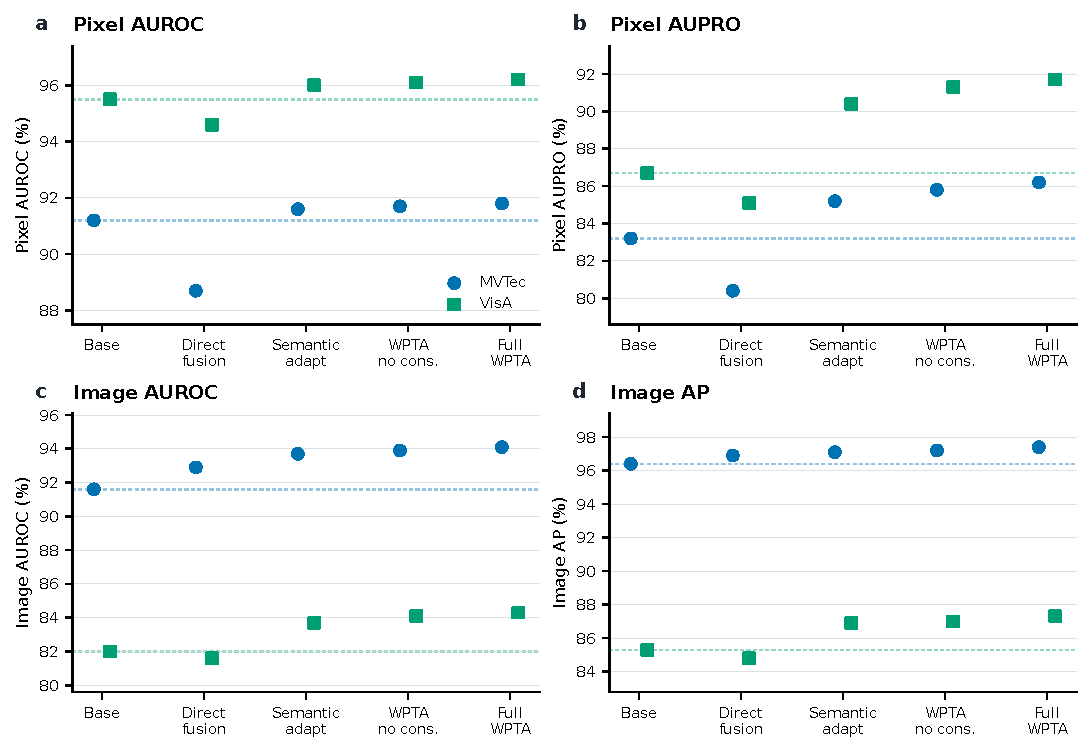
\includegraphics[width=\textwidth]{figures/figure2_core_ablation.pdf}
\caption{Core component ablation on MVTec and VisA. Each panel reports one evaluation metric for the fixed baseline, direct wavelet fusion without prototype adaptation, semantic-only prototype adaptation, wavelet prototype adaptation without conservative update, and the full method.}
\label{fig:core-ablation}
\end{figure*}

\begin{figure}[t]
\centering
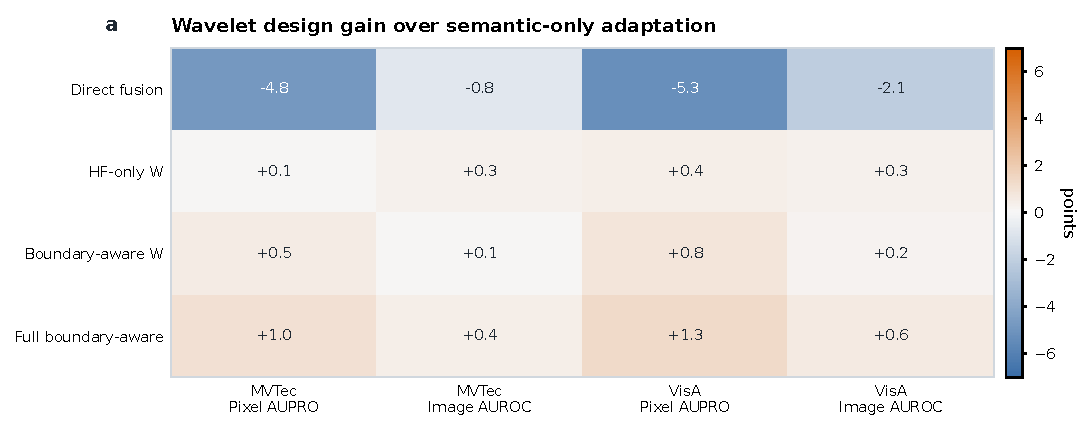
\includegraphics[width=\linewidth]{figures/figure3_wavelet_design_ablation.pdf}
\caption{Wavelet design ablation. Cells show point changes over semantic-only prototype adaptation for pixel AUPRO and image AUROC on MVTec and VisA.}
\label{fig:wavelet-design-ablation}
\end{figure}

\begin{figure*}[t]
\centering
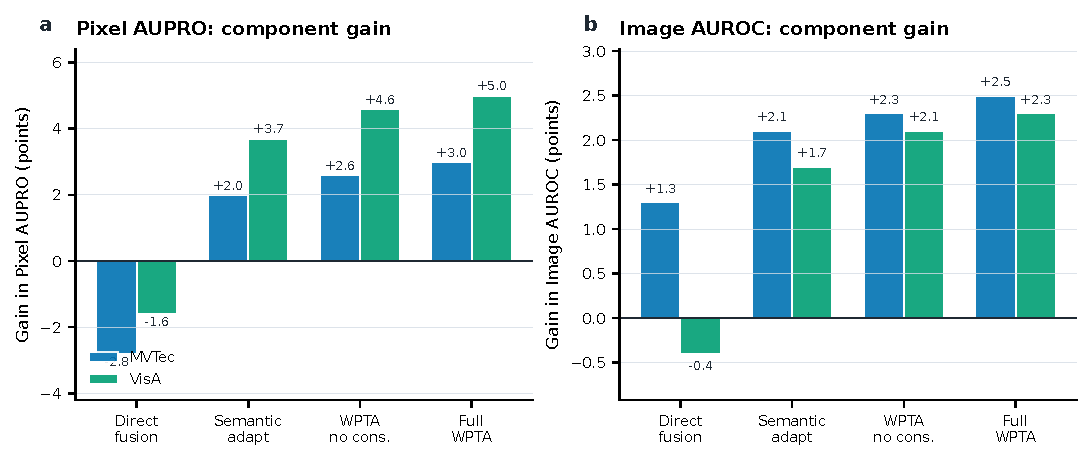
\includegraphics[width=\textwidth]{figures/figure4_core_ablation_bar.pdf}
\caption{Component-level ablation gains over the fixed AnomalyCLIP baseline. Bars report point changes in Pixel AUPRO and Image AUROC on MVTec and VisA.}
\label{fig:core-ablation-bar}
\end{figure*}

\begin{figure*}[t]
\centering
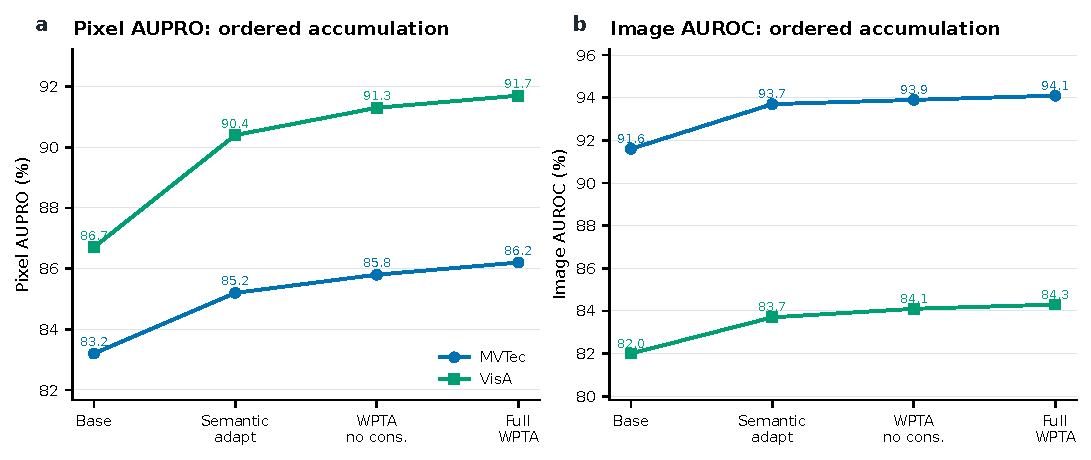
\includegraphics[width=\textwidth]{figures/figure5_core_ablation_line.pdf}
\caption{Ordered component accumulation from the fixed baseline to semantic prototype adaptation, wavelet-guided prototype adaptation, and the full conservative update. Lines are used only for this ordered build-up path.}
\label{fig:core-ablation-line}
\end{figure*}

\begin{figure*}[t]
\centering
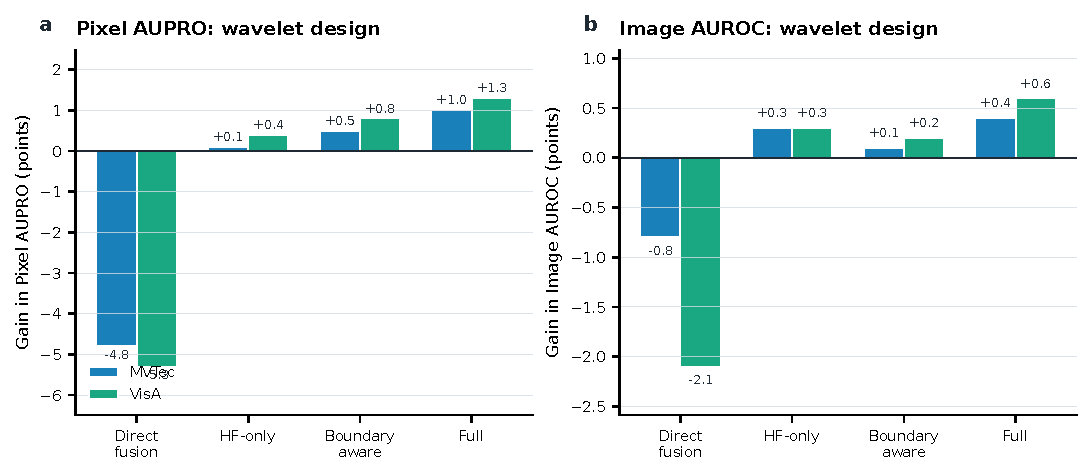
\includegraphics[width=\textwidth]{figures/figure6_wavelet_design_bar.pdf}
\caption{Wavelet design ablation as grouped gain bars over semantic-only prototype adaptation.}
\label{fig:wavelet-design-bar}
\end{figure*}

\begin{figure*}[t]
\centering
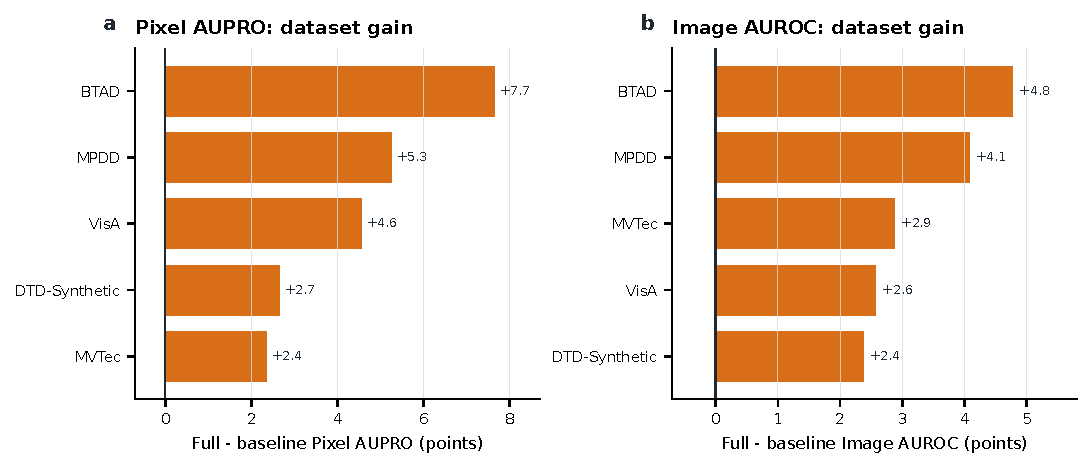
\includegraphics[width=\textwidth]{figures/figure7_main_gain_bar.pdf}
\caption{Dataset-level gains of the full method over the AnomalyCLIP baseline on the two headline metrics.}
\label{fig:main-gain-bar}
\end{figure*}

\begin{figure}[t]
\centering
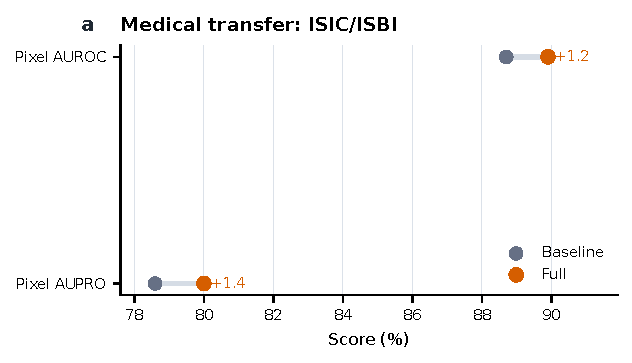
\includegraphics[width=.72\linewidth]{figures/supp_figure_medical_isbi.pdf}
\caption{Supplementary medical transfer result on ISIC/ISBI. Only current completed rows are plotted; blocked medical datasets are excluded.}
\label{fig:supp-medical-isbi}
\end{figure}
